\chapter{Scheduling} % Titlul capotilului
\label{Capitolul4}

\section{Introduction}

In this section we discuss the scheduling problem which consists of choosing the publishing time for every object registered with our library by every application instance. We first identify the requirements on the scheduling algorithm, present some solutions and assess them by using both a simulation and a test-bed deployment of the system.

\section{Monitoring system}

Our monitoring system is composed of approximately 12000 applications which send data to 32 multi-threaded IS servers.  All these applications are instances of 15 binaries, most of them being L2 and EF applications. Instances of the same application have the same set of registered objects.

Since applications talking to different IS servers are independent we analyse them separately. So we consider a system with a single IS server and 400 applications that run on 40 nodes. The communication is done using CORBA \citep{vinoski1997corba} and the server has 8 threads by default and runs on a machine with 12 CPUs. We also assume that the IS server runs in the same rack with the applications that use it and is connected to the same switch with a 1Gbps connection.

A typical example of monitored objects set is the one of the Event Filter nodes which monitor 5138 histograms with an average of 438 bins per histogram. For L2 nodes, there are 5087 histograms with 1126 bins in average. The publishing intervals are usually configured between 1 second and 10 minutes. Although applications publish many other kinds of objects such as counters or flags, most of the published monitoring information consists of histograms. Since histograms have the biggest influence on the performance of the system I will consider only them for the analysis in this chapter.

\section{Requirements}

\begin{description}
\item[Minimize jitter.]

First of all, we should be able to publish each histogram periodically, with the interval between two consecutive publications approximately equal to the interval configured by the user. We should be able to handle multiple publishing intervals. A number of intervals of the order of 10 is expected.

Let's consider a histogram with publishing interval $I$ and let the time of the $k$-th publication of a histogram be $T_k$; we call $J=\max(\lvert T_k-((k-1) \cdot I+T_1\rvert))$ the jitter of the histogram. We want to have $J < 0.1\cdot I$ for every histogram.

\item[Minimize latency.]

We publish the histograms using a separate thread from that of the main application which does the event filtering. In this thread we call a black-box function that takes care of all the details of sending the histogram to the IS server (buffering, marshaling, etc.). We have to keep the histogram locked while we are calling this function in order to prevent a concurrent modification from the thread that is updating the histogram. As the main application thread may block waiting for the histogram to be published instead of doing useful work, we want to minimize the publishing latency.

\item [Minimize publishing skew.]

Collision event data is distributed to all the applications, each maintaining its own histograms about the processed events. These histograms are evolving in time and in order to have an overview about the system's operational state we need to take a snapshot of the histogram instances from all nodes at some point in time and to aggregate them.

In order to take a snapshot of histogram instances across all nodes at some point in time, we need to have all nodes publishing their instance of that histogram with minimal skew. The publishing skew of a histogram is defined to be the difference between the moments when the first and the last instance of the histogram is received by the IS server.  

\item [Maximize throughput]

We want the published information in the IS server to be as fresh as possible. So we need to publish as many histograms per second as possible allowing the user user to configure small publishing intervals.

\item [Efficient incremental reconfiguration]

We want to allow the users to reconfigure the system at runtime, which means that our schedule should incorporate the new changes on the fly. We want to implement this feature as efficient as possible which means we don't want the system to stop publishing for a long time in order to apply the new configuration changes. 

We also want that if we change the publishing interval for some histograms, the rest of them should continue to be published according to the existing schedule.

\item [Avoid bursty traffic]

A bursty traffic pattern seen by the IS server impacts the overall system performance in multiple ways. First, it requires big inbound queues in IS server, networking devices and in all the upstream applications to which the IS server pushes information. 

Another effect is related to the IS subscriber applications that use garbage collection for memory management, for example \citep{sicoe2012persistent}. They are known to suffer from freezes when a stop-the-world garbage collector runs \citep{aho2007compilers}. However, more recent garbage collection algorithms \citep{printezis2005garbage} are designed to work in parallel with the application as long as it doesn't allocate memory at a very high rate which is exactly what bursty traffic causes.

Although important, this requirement has the same cause as the first one, namely contention, so we will treat it as a secondary one.

\end{description}

\section{Global and local scheduling}

The previously identified requirements can be split into two classes. The first class consists of the requirements that can be satisfied by each application instance in isolation; we call them local requirements. These are jitter minimization and reconfiguration efficiency. 

The second class consists of requirements like skew and latency minimization and bursty traffic avoidance which are global requirements that can be satisfied only if the application instances cooperate. Although the instances of applications that use the monsvc library do not communicate explicitly, they affect each other’s performance when creating contention in the monitoring network of the ATLAS TDAQ system. 

In order to treat the two classes of requirements more orthogonally, we consider the time as being divided in equal length slots. This way we can think of local scheduling as assigning which histograms are published in which slot and the global scheduling as when to publish the histograms within a time slot.

The slot size choice is not simple since it has conflicting requirements, but on the positive side it does not depend on the library configuration, so it has to be changed only when there are big changes in infrastructure (hardware and network) or when the distribution of histograms sizes changes fundamentally.

This separation also helps us in presenting to the users a simple model for configuring the publishing intervals. The system reports the number of available slots per second and the users need just to calculate how many slots per second their rules require. The users, however, should not expect 100\% utilization of the slots due to irregularities of the publishing intervals set.

\section{Global scheduling}

For this problem we assume that we every application has the same set of histograms to publish in a particular time slot. The set of histograms is very small, ideally only one histogram, but due to the imperfection of the local scheduling there can be several of them.

We have to satisfy two conflicting requirements, namely publishing skew and latency minimization. In order to minimize publishing skew we should try to make all the applications publish simultaneously. But this practice will create contention in the network and in the IS server and the latency will increase. 
The strategy that we adopted for this problem is to make each application choose the moment of publishing randomly within the first part of the time slot of length $f\cdot I$, where $f<1$ is a configuration parameter and $I$ is the size of the time slot. We call the length of this first part of a time time slot \emph{initial delay bound}.

In order to deal with the case in which the time slot is too short for publishing all the histograms, we extend it until we are done publishing everything and reduce the length of the next interval.

An example of scheduling is depicted in figure \ref{fig:local_sched}, where we have three applications that start the publishing within the first $f=0.75$ part of the interval.

\begin{figure}[ht!]
\centering
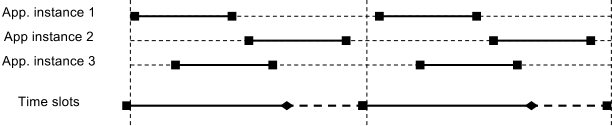
\includegraphics[scale=0.6]{Images/local_sched.png}
\caption{Global scheduling example.}
\label{fig:local_sched}
\end{figure}

Since we have no communication between applications our solution has a very low overhead and is fault tolerant. It is also robust with respect to the clock skew as long as it is small enough (of the order of 1ms). Another advantage is that by tuning the $f$ parameter we can trade-off between skew and latency. 

\section{Real-time formulation of local scheduling}

The local requirements for our scheduling requirements can be viewed as a real-time scheduling problem \citep{liu1973scheduling}, \citep{sha2004real}. In order to make this more apparent, we establish the following mapping of concepts:
\begin{itemize}
\item Each \emph{histogram} is considered a {\bf task} that generates jobs periodically. An application instance registers $n \approx 5000$ histograms.
\item A {\bf job} consists of publishing the \emph{histogram} to the IS server.
\item The \emph{latency} of a publishing a histogram corresponds to the {\bf execution time} of a job $C_i$. 
\item The \emph{publishing interval} is the {\bf task period} $T_i$. A typical configuration include $m=5-10$ distinct periods which are integer numbers of seconds and usually less than 10 minutes.
\item The \emph{maximum jitter} of a histogram is the {\bf deadline} of the corresponding job $D_i=0.1\cdot T_i$.
\item The \emph{IS server} has a similar role to the {\bf CPU} that need to be scheduled among the tasks.
\item The \emph{throughput} of our system is the {\bf utilization} $U$ of the corresponding real-time system.
\end{itemize}

\subsection*{Related work}

In the real-time scheduling literature there are two main classes of algorithms: static ones in which the priority of a task is determined before the system is started and dynamic ones in which the priority of a task is adjusted dynamically. 

The most widely used static algorithm is the Rate Monotonic Scheduling (RMS) \citep{liu1973scheduling} in which the priority of a task is higher for tasks with small periods. The algorithm is preemptive, so when a task with small period becomes available, the ones with larger period are preempted and it starts running. Another variation is Deadline Monotonic Scheduling which gives higher priority to tasks with shorter deadlines. In our case, we cannot preempt a histogram that has already started to be published, so this algorithms are not directly applicable. 

Among the dynamic algorithms, we mention Earliest Deadline First (EDF) \citep{liu1973scheduling} in which, whenever the processor is idle and some tasks are available, we start the task whose deadline comes first and run it to completion. This algorithm is optimal in the sense that if a system is schedulable with some algorithm, then it is also schedulable with EDF.

People concentrated on developing criteria to check whether a real-time system is schedulable with these algorithms. For EDF the condition given in \citep{baruah1990algorithms} is that the utilization $U < 1$ and the following holds:

$$ \forall L > 0.\,  \sum_{i=1}^n \left\lfloor \frac{L+T_i-D_i}{T_i}\right\rfloor C_i \le L $$

which in our case, for $C_i=10$ms, $T_i=5$mn, $L=D_i=30$s, $n=5000$, becomes:

$$ \sum_{i=1}^n 1 \cdot C_i \le L \Leftrightarrow 50s \le 30s $$

Note that the utilization in our case is $U=\sum_{i=1}^n\frac{C_i}{T_i}=n\frac C T = \frac 1 6 = 0.166$ which is very low. 

For DMS in order to check the schedulability, we have to determine the worst case response time for every task using the following set of recursive equations \citep{joseph1986finding}.

 $$ \forall i.\, R_i=C_i+\sum_{j=1}^{i-1} \left\lceil \frac{R_i}{T_i} \right\rceil \cdot C_j \Leftrightarrow R_i = i\cdot C$$
 
So, again, the response time for the last histogram is $R_n=n\cdot C=50s > D_n=30s$. We can notice that since all the histograms have the same period they have the same priority so they are published sequentially. Hence, in order to satisfy the deadlines with this algorithm we should be able to publish all the histograms in 10\% of the time. Note that having higher priorities for some of the histograms does not improve the situation of the ones with low priority.

\subsubsection*{Offset-free systems} 

The common assumption of these algorithms that render them ineffective for our system is that all histograms should start to be published in time slot 0. However, this is not necessary in our case, so, we have more degrees of freedom in choosing the time offset at which the first publication of each histogram occurs. Multiple choice strategies are presented in the literature about offset-free systems \citep{goossens2003scheduling}, \citep{grenier2008pushing}.
 
In \citep{goossens2003scheduling} the author proves a number of useful results about offset-free systems and presents two algorithms for assigning offsets to a set of tasks. The first algorithm finds an optimal offset assignment and it has a running time of $O(n^2 \cdot \frac{\prod_{i=1}^n Ti}{\text{lcm}(T_i)})$ which renders it useful only for theoretical purposes. The second algorithm is an heuristic one which runs in $O(n^2\cdot \log(\max_{i=1\ldots n}(T_i)))$ and has space complexity $O(n^2)$. The algorithm works by considering pairs of tasks in decreasing order of greatest common divisor of their periods and trying to assign offsets such that the jobs of these two tasks are as distant as possible. The limitation of this algorithm is that it looks exactly at one other task offset before choosing the offset for a task.

In the context of scheduling messages in CAN networks, Grenier et al. \citep{grenier2008pushing} propose another heuristic algorithm which runs in $O(n\cdot \max_{i=1 \ldots n}(T_i))$ and has better experimental results than the previous one. The algorithm tries to assign offsets such that the first job of every task is as far as possible from other jobs. It does this by considering tasks in the increasing order of their periods and assigns the offset such that the first job of task is as far as possible from every job of a task that was assigned so far. The drawback of this approach is that the algorithm does not look at the subsequent jobs of a task and it creates collisions (two jobs scheduled for the same time) even for simple scenarios.

Once the offsets have been chosen, we still have to design a scheduling algorithm. For offset-free systems, the DMS algorithm is no longer optimal among static algorithms but an optimal priority assignment can be found with $O(n^2)$ time complexity \citep{audsley2001priority}. On the other hand, among dynamic algorithms EDF is still optimal. 

\section{Hash based offset assignment}

A simple offset assignment algorithm chooses the offsets by hashing the names of the histograms and taking the value modulo their period. In order to have histograms with different names published with small skew one can configure an identical \emph{hashing name} which, if present, is used instead of the histogram name to determine the time slot 

This strategy ensures that every application will assign the same offset to a histogram even if they have different histogram sets to be published. However, this situation can only occur when we change the configuration at runtime and only for brief periods. Another positive aspect is that the reconfiguration can be done in $O(1)$ time: we just assign offsets to the changed histograms and keep the existing ones unchanged.

The problem of this algorithm is that even for a perfect hashing function the expected maximum number of histograms assigned to a single slot is $O(\frac{\log n}{\log \log n})$ \citep{mitzenmacher1996power}. They will overload the IS server, will overflow to the next time slots and increase the publishing skew. On the other hand, the expected number of empty slots is $\frac n e$ which gives us a throughput of 63\% of the maximum.

\section{Subperiod offset assignment algorithm}

In this section we present a heuristic algorithm that leverages the particularities of our system to assign offsets for histogram with no jitter, no collisions and high throughput. 

In our configuration files, all the periods are expressed in seconds which means that the greatest common divisors among periods are large - equal to the number of slots per second which is 30-100. Moreover, large subsets of histograms have periods which are multiple of 5 or 10 seconds. We will also take advantage of the fact that we have only a few (5-10) distinct periods in order to achieve better time complexities for offset assignment.

\subsection{Conventions}

It is proved in \citep{goossens2003scheduling} that we can choose the offset for a histogram to be less than its period without loss of generality. 

In the context of a single histogram, its offset determines a set of slots. For example, an offset $k$ for a histogram with period (i.e. publishing interval) $P$ represent the slots $\{k+n\cdot P | n \geq 0\}$. Note that in the definition, the period was implicitly defined by the histogram. If the period cannot be derived from the context, we explicitly mention it: offset $k$ modulo $P$.

\subsection{Intuition and pseudocode}

The algorithm operates in two steps. First it repeatedly approximates unions of histogram groups with different periods with one group having a smaller period until we are left with only one group. Then we start with this group and assign offsets recursively to groups that it approximates until we get to assign offsets to all histograms.

At the beginning every histogram will form its own group:
\begin{verbatim}
group = {period : histo.period, n : 1, offset : None}
\end{verbatim}
In order to describe the approximation operation let’s take an example configuration which includes two histogram groups: one having 4 histograms to be published every 10 sec. and another one 4 histograms to be published every 15 sec. So, we need to assign 4 offsets in the range [0s, 10s) and 4 offsets in the range [0s, 15s).
 
Let’s consider the time being divided in 5 sec subperiods. Denote by x the number of offsets from the first group that are chosen in the interval [0s, 5s) and by y the number of those in the interval [5s, 10s). Similarly, denote by a, b, c the number of offsets from the second group in the three 5 seconds subperiods of the interval [0s, 15s). In the figure \ref{fig:subperiod} we represented the number of slots used to publish histograms in 6 consecutive subperiods of 5 sec:

\begin{figure}[ht!]
\centering
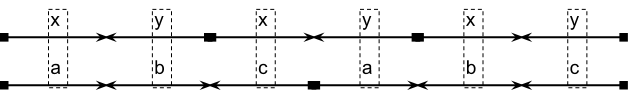
\includegraphics[scale=0.6]{Images/subperiod.png}
\caption{Distribution of the histograms among subperiods.}
\label{fig:subperiod}
\end{figure}

We have a fixed number of slots per second, so we have a bound on the number of slots that we can use in each of the subperiods. In order to stay within this bound our strategy is to minimize the maximum number of slots used in a subperiod. In our case this reduces to the following optimization problem:
$$ \text{minimize } \max(x+a, y+b, x+c, y+a, x+b, y+c) \text{ subject to } a+b+c=4 \text{ and } x+y = 4 $$
One can easily prove that:
$$ \max(x+a, y+b, x+c, y+a, x+b, y+c) = \max(x, y, z) = \max(a, b, c)$$
So, we only need to minimize the maximum number of slots used in a subperiod for each of the two task groups. The minimum of 4 slots is achieved if we distribute the offsets uniformly among subperiods of 5 sec, that is, choosing $x=2, y=2$ and $a=2, b=c=1$. With this setting we can (over-)approximate the union of the two groups with one (synthetic) group of 4 histograms to be published every 5 sec.

In general the following function computes the approximation of two groups:
\input{Code/approximate}
The \verb+sons+ field stores the groups that it approximates together with their maximum number of slots per subperiod.

This is an over-approximation in the sense that if we can assign offsets (without collisions) for the resulting group, then we can also assign offsets for the initial groups. Let’s assume we have assigned offsets $\{o_1,o_2,o_3,o_4\}$ to the four histograms in the synthetic group. We can allocate offsets $\{o_1, o_2\}$ modulo 5 sec for the first group and offsets $\{o_3, o_4\}$ modulo 5 sec. Note that these offsets are the same with $\{o_1, o_2, o_1 + 5, o_2 + 5\}$ modulo 10 sec and $\{o_3, o_4, o_3 + 5, o_4 + 5, o_3 + 10, o_4 + 10\}$ modulo 15 sec. These two offset sets can now be recursively assigned to the 4 histograms in each of the groups. The general algorithm is presented in pseudocode below:
\input{Code/assign}
The next function converts the offset list from offsets modulo subperiod to offsets modulo \verb+period+:
\input{Code/expand}
A sketch of a possible algorithm execution is presented in figure \ref{fig:subperiod_tree}, where we have 5 histograms with period 2 sec, 4 histograms with period 10 sec. and another 4 histograms with period 15 sec. The blue rectangles represent the initial histograms and the purple ones represent approximating groups. The strategy of choosing the next pair of groups to approximate determines the shape of the tree.
\begin{figure}[ht!]
\centering
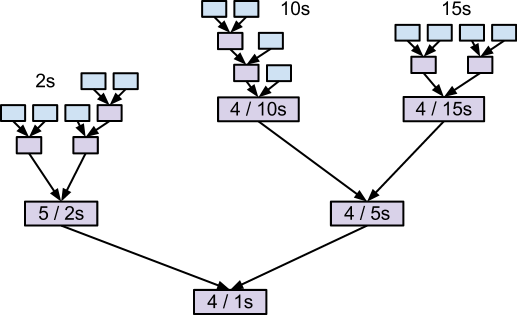
\includegraphics[scale=0.7]{Images/subperiod_tree.png}
\caption{Subperiod tree.}
\label{fig:subperiod_tree}
\end{figure}

Now we just need to assign offsets to the root group and they will be pushed towards the leafs:
\begin{verbatim}
assign(build_tree(groups), root_offsets)
\end{verbatim}

\subsection{Incremental version}

In the algorithm presented above we assign a set of offsets to the root group of the tree which takes care of pushing subsets of it to its children nodes, which recursively push subsets of them up the tree until they reach the leafs where they are assigned to histograms. A node may not be able to push all its offsets to the children, thus leaving unused offsets along the way. For example, in order to assign 4 offsets to the group with period 15 sec we need to allocate 2 slots modulo 5 sec. from the parent node that actually which actually mean 6 offsets modulo 15 sec leaving us with 2 unused offset modulo 15 sec.

When a new histogram is added, it is attached to the tree as a leaf. Next, we should locate some unused offsets in the tree and try to push them towards the newly added node. However, it is simpler to use a pull model in which the node corresponding to the newly added histogram is pulling an unused offset from its parent. If the parent has no unused offsets, it tries to pull some from its parent and so on, until the root is reached. At this point algorithm fails if there are no unused offsets.

We associate an {\tt OffsetSupply} to each of the nodes to hold its unused offsets. Initially all the supplies are empty except from the root whose buffer is pre-filled with all the offsets modulo its period. When a node pulls an offset from its parent supply, it converts it to multiple offsets modulo its period.
\input{Code/offsetsupply}
The algorithm for adding a histogram is the following:
\input{Code/addhisto}
If this incremental addition of a histogram to the tree with pull-based offset assignment succeeds, the previously assigned offsets are preserved. However, this incremental changes to may determine a sub-optimal tree structure. So, if the algorithm fails, as a last resort, we rebuild the tree from scratch and possibly change all previously assigned offsets.

\subsection{Complexity analysis}

In this section we will discuss the trade-off between the complexity of the strategy to choose the next pair of groups to approximate and the quality of the resulting offset assignment.

Let’s first introduce a quality measure for a subperiods tree built by our algorithm. 

\begin{definition}
For a node with period $P$ whose parent node has period $P_1$ we define the maximum number of offsets modulo 1 sec. wasted along the edge between the two nodes to be $c(P_1,P)=\frac{1}{P_1}-\frac 1 P$.
\end{definition}

This maximum is achieved if the child pulled a slot from its parent, so it reserves $\frac P {P_1}$ slots modulo $P$, and delivered only one slot to its children. This means $\frac P {P_1}-1$ wasted slots every $P$ seconds, which is $\frac 1 {P_1}- \frac 1 P$ wasted slots per second. 

\begin{definition}
The total maximum number of unused slots for a tree is $c(T)=\sum_{e\in T}c(e)$. 
\end{definition}

For convenience we call these numbers the cost of an edge and of a tree respectively. A strategy is better than another one if it produces trees with smaller cost. 

Note that this measure is very conservative. First because we assume that the worst case happens for every edge which usually is not the case. Second, because these slots are wasted by our algorithm when compared to a hypothetical assignment that uses $\frac 1 P$ slots every second to publish a histogram with period $P$. Even an optimal schedule that satisfies the deadlines of our system leaves some slots unused compared to this hypothetical schedule. Finally, these slots are not entirely wasted - they can be used when we add new histograms incrementally.

\subsubsection*{NP-hardness of optimal subperiod tree}

Equipped with these definitions, the problem of building an optimal tree for $n$ histogram groups with periods $P_1, P_2, \ldots,P_n$ can be formulated as follows. 

\begin{problem}[Optimal Subperiod Tree]
Let’s consider the graph with vertices denoted by numbers $1,2,\ldots ,P$ where $P=\max_{i=1,\ldots,n}(P_i)$ with an edge between vertex $b$ and vertex $a$ of cost $\frac 1 b -\frac 1 a$ iff $b \vert a$. Find the minimum-cost \emph{subperiod tree}, that is, the minimum-cost tree that has leafs $P_1,\ldots,P_n$ and root $\gcd(P_i)$.
\end{problem}

We can notice that this problem is an instance of the Directed Steiner Tree optimization problem which is NP-hard and the with standard complexity assumptions there exists no approximation algorithm with a ratio better than $\frac {\ln (n)} 4$ \citep{zelikovsky1997series, ming2006fasterdsp}.

We will prove that our problem is also NP-hard by reducing from the Bounded Frequency Set Cover problem \citep{gary1979computers, cmulecture}. Actually, since our problem has numeric inputs we will prove it strongly NP-hard \citep{garey1978strong}, that is, it is NP-hard even if the numeric inputs, i.e. the periods, are bounded by a polynomial in the input size.

\begin{problem}[Bounded Frequency Set Cover] Let's consider a finite set $X=\{x_1,\ldots,x_q\}$ and a collection of its subsets $C=\{C_1,\ldots, C_n\}$ such that each $x_i$ occurs in at most $B$ of these subsets, where $B \geq 2$. Find the smallest $k$ such that there exist a subcollection of $C$ of size $k$ that covers the set $X$?
\end{problem}

Let's first assume without loss of generality that there is no element $x_k$ which belongs to every subset $C_i$. If it does, we can remove them from $X$ and from all subsets and the resulting problem is equivalent.

Now, let’s present the polynomial time reduction from the Bounded Frequency Set Cover problem to Optimal Subperiod Tree problem. Let's associate with every $C_i$ a prime number $p_i$ and with every $x_i$ the number $P_i=\prod_{x_i\in C_k}p_k$.

We can choose $p_i$ to be the $2\cdot r+i$-th prime number, so according to \citep{jaroma2005upper} it will satisfy $2\cdot r <p_i<2\cdot 3r \ln 3r$ where $r=\max(n, q)$ and we will be able to bound the periods by a polynomial in the input size, for example $P_i=O(r^{B+1})$. In order to establish the reduction between the corresponding decision problems we prove the following theorem. 

\begin{theorem}\label{theorem}
There exists a subperiod tree in the given graph which has the cost between $k-0.5$ and $k+0.5$ if and only if the BFSC instance has a subcover of size $k$ for $k \ge  1$.
\end{theorem}

First we prove an useful lemma which says that the cost of a closed subtree is small when its root is small. We call a subtree closed if it contains all the descendants of its root that belong to the tree. 

\begin{lemma}\label{lemma1}
The cost of a closed subtree that contains $k$ leafs and whose root is $p$ has the cost at most $\frac{k}{p}$.
\end{lemma}

\begin{proof}
We proceed by induction on the number of nodes. If there is only one node, it is a leaf and the cost of the tree is $0<\frac 1p$. Otherwise, the root has two children with periods $p_1$ and $p_2$ that have $k_1$ and $k_2$ leafs in the corresponding subtrees. The cost of the tree is: 

\begin{eqnarray*}
c(p) &=& \left(\frac 1p - \frac 1 {p_1}\right) + \left(\frac 1 p - \frac 1 {p_2}\right)+c(p_1)+c(p_2) \\
    &\leq & \frac 2p-\frac 1 {p_1}-\frac 1 {p_2} + \frac {k_1}{p_1}+\frac {k_2}{p_2} \\
    &=&\frac 2p + \frac{k_1-1}{p_1}+\frac{k_2-1}{p_2} \\
    &\leq & \frac{k_1+k_2}p \\
    &=&\frac kp
\end{eqnarray*}

We applied the induction hypothesis for the subtrees rooted at $p_1$ and $p_2$ which have fewer nodes. 
\end{proof}

\begin{lemma}\label{lemma2}
If in a subperiod tree with root 1 in which the root has exactly $l \ge 1$ neighbours the cost belongs to the interval $(l-0.5,l+0.5)$.
\end{lemma}
\begin{proof}
The cost of the edges between the root and its neighbours is $c_1$ where $c_1 \le l$ and 

$$c_1 = \sum_{j=1}^{l} 1-\frac 1 {p_{i_j}}  = l - \sum_{j=1}^l \frac 1 {p_{i_j}} \geq l-\frac l {2r} >l-0.5$$

According to the lemma \ref{lemma1}, the cost of the edges in the rest of the tree is $c_2$ where $c_2 \ge 0$ and 
$$c_2 \le \sum_{j=1}^l \frac 1 {p_{i_j}} \leq \frac l {p_1} < \frac r {2r} < 0.5$$

So, the total cost of the tree is between $l-0.5$ and $l+0.5$.
\end{proof}

\begin{proof}[Proof of Theorem \ref{theorem}]
The root node of the subperiod tree is the node 1. Otherwise, it means that all the $P_i$ have a common prime divisor (a divisor of the root) which correspond to an element $x_k$ which belongs to all subsets $C_i$. Contradiction.

Since the number of leafs in the subperiod tree is $q$, the root of the tree has at most $q$ neighbours.

We will prove the two parts of the equivalence between the two implications of the theorem separately:

\begin{description}
\item[($\Rightarrow$)] 
Let's denote the number of neighbours of the root of the tree by $l$. So, the cost of the tree belongs to $(l-0.5, l+0.5)\cap (k-0.5,k+0.5)$ and the only case in which this set is non-empty is when $l=k$.

Let $D_1, \ldots, D_k$ be the neighbours of the root. For each of them, the leafs in its subtree are divisible with $D_i$, so they are divisible with one of its prime divisors $p_{i_j}$, so they are contained in $C_{i_j}$. Hence, the subcollection $C_{i_j},j=1,\ldots,k$ is a subcover of size k.

\item[($\Leftarrow$)] Let $C'=\{C_1,\ldots,C_k\}$ be a subcover of size $k$. Let's consider the tree $T$ with edges 
$$E = \{(1, p_i) \,|\, i=1,\ldots, k\} \cup \{(p_i, P_j) \,| \,\, p_i | P_j\}$$

Since $C'$ is a subcover it means that $\forall j. \exists i. x_j \in C_i$ which means that $\forall j. \exists i. p_i \vert P_j$, so every $P_j$ is an endpoint of an edge in $E$. So, $T$ is a subperiod tree. According to the lemma \ref{lemma2} the tree has the cost between $k-0.5$ and $k+0.5$.

\end{description}\end{proof}

Now we state the reduction form Bounded Frequency Set Cover to the Optimal Subperiod Tree.
\begin{theorem}[BFSC to OST reduction]
The optimal subperiod tree in the given graph has the cost in the interval $(k-0.5, k+0.5)$ if and only if the smallest subcover of the BFSC instance has size $k$.
\end{theorem}

\begin{proof}
Apply theorem \ref{theorem}.
\end{proof}

Following the same lines we can prove that even a strategy that chooses a minimal number of neighbors for the root is NP-hard to find.

\subsubsection*{Heuristic strategy}

In this section we will present a heuristic strategy to compute a near optimal subperiods tree for practical cases with reasonable complexity. 

A first step is to approximate not only pairs of groups but also multiple groups with the same period. It is easy to see that all k histograms with period $P$ can be approximated (exactly) by a group of $k$ histograms with period $P$. Before building the tree we can create these groups in $O(n)$ leaving us with only $m$ nodes to be processed by the \verb+build_tree+ function. 

In the \verb+build_tree+ function we consider the pairs of groups in decreasing order of their common subperiod. In order to implement this function efficiently we use a priority queue:

\input{Code/build_tree}

Since we have $m$ groups of histograms at the beginning, we end up with $2m-1$ groups in the entire tree. So, the number of pairs inserted in the priority queue is at most $O(m^2)$ since we don’t insert the same pair twice. The number of removals is at most as big, and the number of times the maximum is popped is $O(m)$ since we have at most $m$ iterations in the while loop. The complexity of each of these operations is $O(\log m^2+\log T)$, the second term coming from the $\gcd$ computation. So, the total complexity of the \verb+build_tree+ function is $O(m^2(\log m + \log T))$. 

\subsubsection*{Offset assignment complexity}

For the complexity analysis of the offset assignment we will use the pull version presented in the previous section. We assume that the offset buffer of the \verb+OffsetSupply+ is built lazily, so its construction and pop operation are $O(1)$. I also assume that in $O(m)$ we merge all nodes with their parents that have the same period.

Let’s estimate the cost of making $k$ pull operations from the offset supply $s$. Let's denote its ancestors by $s_i,i=1,\ldots,l$ and let the period of $s_i=d_1\cdot\ldots\cdot d_i$ where $d_1=1, d_i \geq 2$. It is easy to see that the pull operations from the offset supply $s_i$ will have to call the pull method of $s_{i-1}$ every $d_i$-th time. We can easily the following recurrence for the cost of $k$ pull operations on the node $s_i$.

$$ f(s_i, k) = k + f\left(s_{i-1}, \left\lceil \frac k {d_i} \right\rceil \right)$$

The solution of this recurrence is:

\begin{eqnarray*}
f(s_l,k) &=& k+ \left\lceil \frac k {d_l} \right\rceil + \left\lceil \frac k {d_l\cdot d_{l-1}} \right\rceil + \ldots + \left\lceil \frac k {d_l\cdot \ldots d_2}\right\rceil \\
         &<&l+k+\frac k {d_l}+ \frac k {d_l\cdot d_{l-1}} + \ldots \\
         &\leq & l+k+\frac k 2+\frac k 4 + \ldots \\
         &<& m+2k
\end{eqnarray*}

So, the complexity of all $n$ pull operations from $m$ offset supplies associated with $m$ distinct nodes is $O(m^2+n)$ and the complexity of an incremental change which adds $k$ histograms with the same period is $O(m+k)$. 

\subsection{Scheduling algorithm}

We use an EDF scheduler which in our case has to return the histogram that needs to be published in the next time slot. In order to speed up the scheduling decisions we split histograms into groups according to their period and sort them by offset inside each group. 

\subsubsection*{Heap-based scheduler}

One possible implementation of the scheduler is to use a min-heap to hold the next histogram to be published from each group, ordered by the earliest deadline. After a histogram is popped from the heap, the next one for that group is added. This approach has a complexity $O(\log m)$ per scheduling decision which is low enough for our purpose. The space complexity is $O(m)$.

\subsubsection*{Table-based scheduler}

We can implement the scheduler with only $O(1)$ time complexity per scheduling decision at the price of higher space complexity. The classic approach is to precompute the schedule for a time duration equal to the least common multiple of the periods. Since we do not have collisions, we can improve over this approach by storing only a small window of the future schedule as a circular buffer. The schedule decision consists of removing and returning the histogram at the beginning of the buffer and adding the next histogram from the same group at its corresponding position.
 
The buffer size is equal to the greatest interval between two offsets of histograms having the same period. This is  $O\left(\max\left(\frac {T_i}  {n_i}\right)\right)$, where $n_i$ is the number of histograms in the $i$-th group, so it is at least $O(\max_{i=1,\ldots,n}(T_i))$.

\subsubsection*{Incremental schedule changes}

While making changes to the histogram configuration, the system continues to publish the histograms with the old schedule. Meanwhile, we assign the new offsets in another thread using the previously described algorithm. Only when the new offset assignment is computed, we briefly stop the scheduler to make the changes.

This technique allows us to have smooth incremental changes even when the subperiod tree is rebuilt - process that runs in time $O(n+m^2(\log m+\log T))$. The actual complexity of changing the table-based scheduler is $O(m)$ for a complete offset reassignment and $O(1)$ for incremental changes. For the heap-based one, the times are $O(m\log m)$ and $O(\log m)$ respectively.






\section{Experimental results}

In order to evaluate the scheduling algorithm and different parameter values, we implemented an event-based simulation tool using SimPy \citep{simpy}. The simulation results were compared with the results of a testbed deployment of the system. Using a simulation allowed us to prototype and evaluate faster and also offered us an easier way to measure values such as server queue length that were not accessible in a testbed deployment.

\subsection{Simulation}

The workload used for comparison consists of the histograms published by the Event Filter nodes: 5138 histograms with 438 bins in average and a publishing interval of 1 minute for all of them. At the extreme, there are two histograms with 178.400 and 228.352 bins. The distribution of sizes (number of bins) is given by the figure \ref{fig:histosize}.

\begin{figure}[ht]
\centering
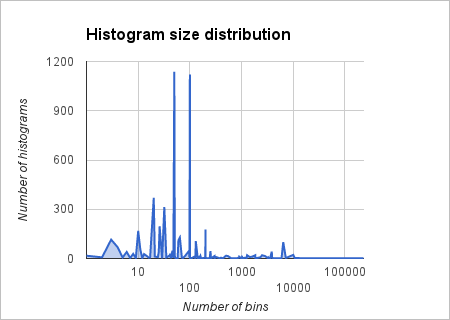
\includegraphics[scale=0.6]{Images/histo_distrib.png}
\caption{Histogram size distribution.}
\label{fig:histosize}
\end{figure}


The model of the publishing process of a histogram has four steps: 
\begin{description}
\item [Preparing the histogram in the CORBA buffer]
The time taken by this step is dependent on the histogram's number of bins. If the histogram is over 2000 bins, a compression algorithm is applied. This is also the longest of the four steps.

Experimental measurements lead us to the following approximating formula:
\begin{itemize}
\item 500 us + \# bins $\times$ 0.05 us, if bins $<$ 2000
\item 1.4 ms + \# bins $\times$ 0.33 us, otherwise 
\end{itemize}
\item[The histogram is sent over the network]
The time is roughly independent of the number of bins, except for very big histograms and is equal to an intra-rack round-trip time = 0.2 ms
\item[The histogram is stored by the IS server]
This step depends slightly on the compressed size of the histograms and takes 0.1 - 0.4 ms. We used as a model for the duration of this step: 90 us + size $\times$ 0.0066 us.
\item[Finalizing steps in the sending application]
Takes 0.1 - 0.2 ms and depends slightly on the compressed size of the histograms.
\end{description}

The latencies were chosen to be consistent with experimental latencies measured using {\tt strace} and measuring the interval between system calls corresponding to messages sent over the network. This approach was chosen because the server was treated as a black-box as it was developed by another working group. 

We simulated 40 nodes with 10 applications each, publishing to an IS server which has 8 threads and is assumed that it run on a machine with enough CPUs to allow the threads to run in parallel. The inbound link of the server has 1Gbps.

\subsubsection*{Global scheduling for one slot}

In the first experiment we varied the initial delay bound and observed the effect on the maximum IS server request queue length, latency and publishing skew. 

We used the setup described above and a workload consisting of one or two histograms with the size given by the table \ref{tab:histosize} published in a single time slot. In the table we provided the amount of time required for an IS server thread to process the histogram and the percentage of histograms with similar size in our sample. 

\begin{table}
\centering
\begin{tabular}[ht]{ | l | l | l | }
  \hline                        
  Size & IS processing & Percentage \\
  \hline                        
  S & 100us & 91\% \\
  \hline  
  M & 200us & 8.3\% \\
  \hline  
  L & 400us & 0.6\% \\
  \hline  
\end{tabular}
\caption{Histogram classes used in simulation.}
\label{tab:histosize}
\end{table}

\begin{figure}[ht]
\centering
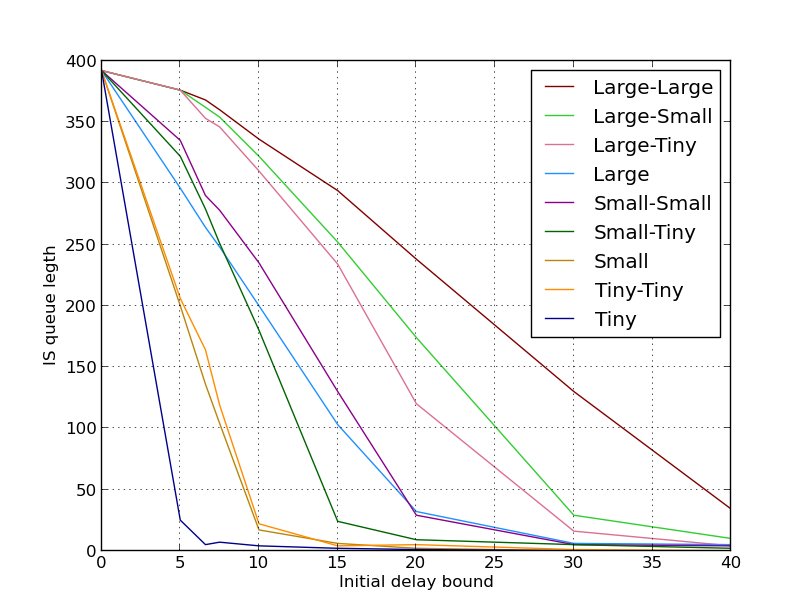
\includegraphics[scale=0.5]{Images/one_slot_sim_qlen.png}
\caption{Maximum IS queue length vs. initial delay bound.}
\label{fig:one_slot_sim_qlen}
\end{figure}

\begin{figure}[ht]
\centering
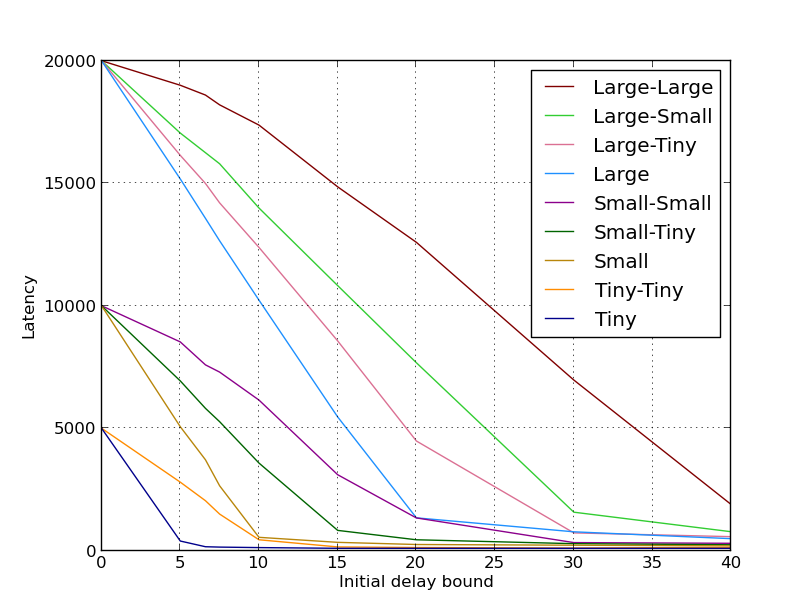
\includegraphics[scale=0.5]{Images/one_slot_sim_latency.png}
\caption{Publishing latency vs. initial delay bound.}
\label{fig:one_slot_sim_latency}
\end{figure}

\begin{figure}[ht]
\centering
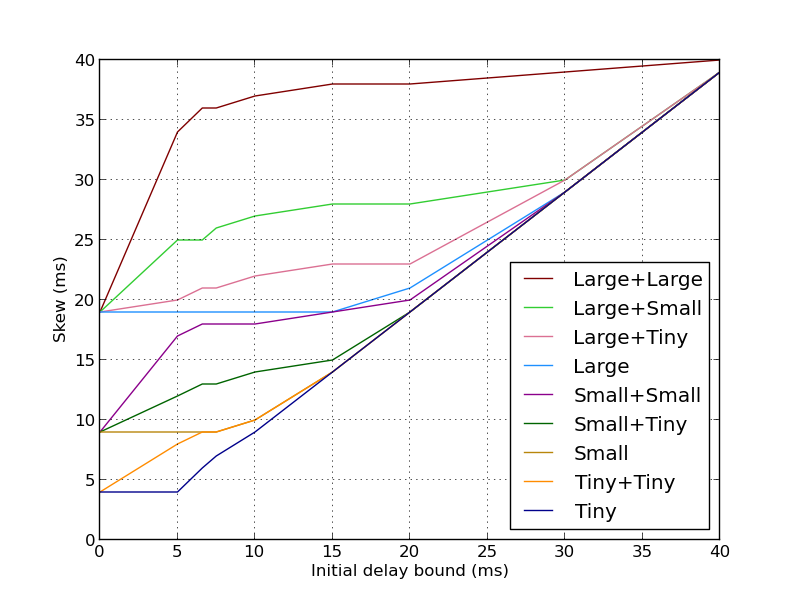
\includegraphics[scale=0.5]{Images/one_slot_sim_skew.png}
\caption{Publishing skew vs. initial delay bound.}
\label{fig:one_slot_sim_skew}
\end{figure}

The results plotted in figures \ref{fig:one_slot_sim_qlen}, \ref{fig:one_slot_sim_latency} and \ref{fig:one_slot_sim_skew} make apparent the inverse relation between publishing skew on one hand and IS queue length and latency on the other hand, both of which we want to minimize. 

Indeed, the IS queue length and the publishing latency decrease significantly with the initial delay bound since we remove their root cause, contention, by randomization. The decrease becomes less steep when the initial delay bound becomes greater than the total time needed to publish all the histograms sequentially. The threshold is equal to the time required to publish all the histograms sequentially by the IS server. For example, 400 large histograms need $\frac {400 \text{ apps}\cdot 400 \text{us}} {8 \text{ threads}} = 20\text{ms}$ and this is exactly where the decrease stops in the graph.

On the other hand, once the initial delay bound is greater than this threshold, the publishing skew becomes roughly equal to the initial delay bound, so it increases in a controlled manner.

\subsubsection*{Global scheduling for multiple slots}

The second experiment aims to study how the global scheduling algorithm behaves over longer periods. We analyse how the algorithm handles the case in which some of the slots are too short for the histograms assigned to them.

To this end we chose a slot size of 15ms and we examined three different assignments of the $\approx 5000$ histogram to $6000$ slots. The first slot assignment is the hash-based one which assigned up to 6 histograms to the same slot leaving approximately 2500 empty slots. The second assignment assigns two histograms per slot in the first slots and leaves the remaining ones empty. The third assignment is an optimal one that assigns each histogram to its own slot. 


\begin{table}
\begin{tabulary}{\textwidth}{|L|L|L|L|L|L|L|L|}
\hline 
Offset assignment & average queue length & stddev queue length & max. queue length & avg. pub. skew (ms) & stddev pub. skew (ms) & avg. latency (ms) & stddev latency (ms) \\
\hline 
 Hash  & 5.72 & 26.0 & 344 & 11.924 & 0.297 & 1.304 & 0.967 \\
\hline
 Pairs & 2.40 & 18.63 & 376 & 11.319 & 0.770 & 1.159 & 0.992 \\
\hline
 Opt.  & 0.28 & 6.57 & 305 & 11.205 &1.699 &1.065 &0.776\\
\hline 
\end{tabulary}
\caption{Offset assignment evaluation during a multi-slot period.}
\label{tab:multi_slot_sim}
\end{table}

We compared the publishing skew, the IS queue length and the publishing latency among three slot assignments and summarized the results in table \ref{tab:multi_slot_sim}. 
\begin{description}
\item[Publishing skew] We can see that it is dictated by the slot length, being approximately 75\% of the interval length. So, it does not change by much for different assignments.

\item[IS queue length]
We can observe an increase both in average and standard deviation when we have multiple histograms per slot. However, the maximum queue length is does not vary by much as it is determined by the slots containing one of the 0.1\% histograms that are have the size 10 times the others. 

\item[Latency]
It is correlated with the queue length and the increase for the hash-based assignment is 25\%.
\end{description}

The conclusion of this experiment is that although the slots will be too short for the very big histograms, a local scheduling algorithm that avoids collisions can reduce latency by 25\%.


\subsubsection*{Subperiod algorithm evaluation}

We have seen that finding the optimal best subperiod tree is an NP-hard problem and we also know that the set cover problem which we reduced to ours cannot be approximated better than a logarithmic ratio. Moreover, there might exist offset assignments that are better than the best one produced by a subperiod tree. In this subsection we show that the subperiod algorithm produces assignments which are close to optimal for practical cases. 

For evaluation purposes, we count the number of slots per second required by our offset assignment algorithm and compare it to the smallest number of slots required if we could use fractional slots. For example, for two histograms with periods 2 and 3, the number of slots required is $\frac 1 2 + \frac 1 3$. This number is clearly a lower bound on the number of slots required by any possible offset assignment, but is not necessarily achievable.

In our experiment most of the periods have only 2, 3 and 5 as prime factors (called \emph{nice} periods) but we allow some other periods also. For several combinations of nice and non-nice periods we ran the algorithm on 1000 randomly chosen inputs and we counted the number of extra slots that our algorithm requires as compared to the above mentioned lower bound. The results are presented in figure \ref{fig:unused_slots}.

\begin{figure}[ht]
\centering
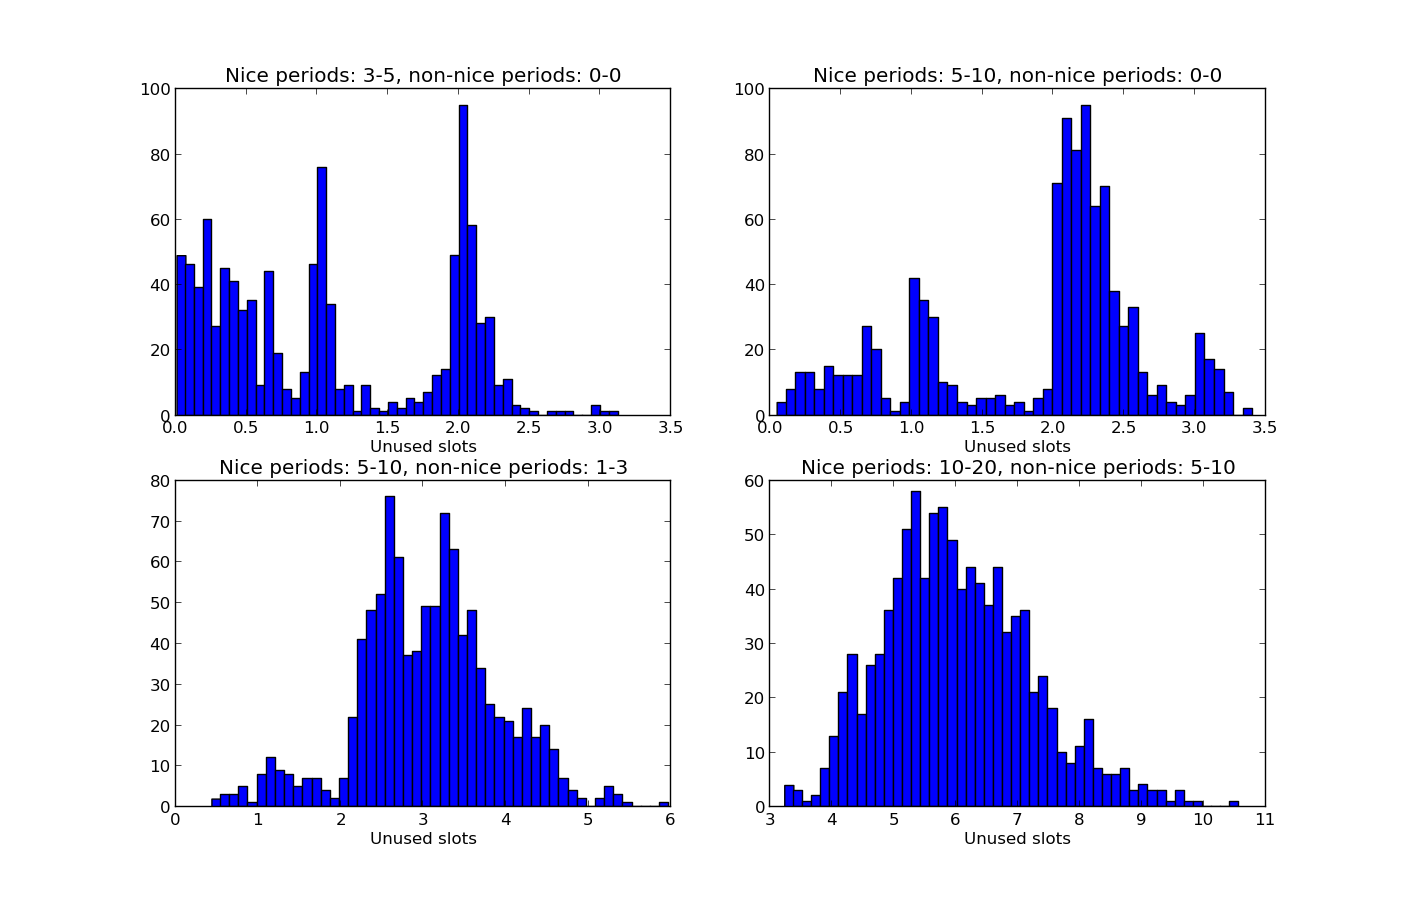
\includegraphics[scale=0.40]{Images/unused_slots.png}
\caption{The number of unused slots by the subperiod algorithm. }
\label{fig:unused_slots}
\end{figure}

In the configuration used in 2012, the configured periods were 5, 10, 20, 40, 60 and 120, so the subperiod algorithm would have left at most one unused slot per second. More generally, for 5-10 nice periods we need only 2.5 more slots than the optimum which is negligible compared to 50-100 slots per second. Even in the extreme case of 10-20 nice periods and 5-10 non-nice we waste at most 20\% of the slots.

\subsubsection*{Throughput, latency and publishing skew}

In the next experiment we evaluated the throughput that can be achieved when using the proposed scheduling strategy: subperiod algorithm for local scheduling and randomization based global scheduling. We tried to vary the slot size and the initial delay bound in order to analyze throughput, maximum publishing skew and maximum latency. 

In the plot \ref{fig:skew_lat_sim} we show the results of publishing the entire set of $\approx 5000$ histograms in $6000$ slots. The initial delay bound is shown as the fraction of the slot size, the rest of the values are expressed in milliseconds. In order to have similar value ranges, the latency is multiplied by 10.

\begin{figure}[ht]
\centering
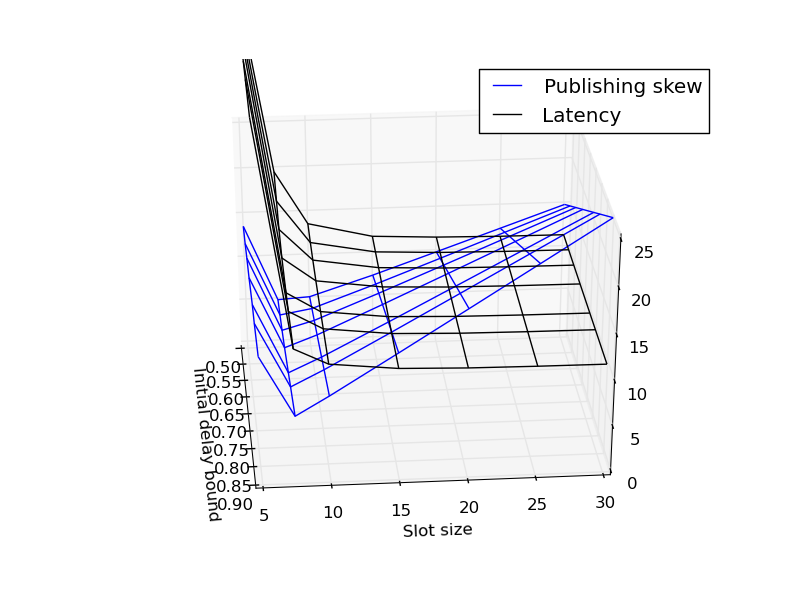
\includegraphics[scale=0.7]{Images/skew_lat_sim.png}
\caption{Skew and latency vs. interval length and initial delay bound.}
\label{fig:skew_lat_sim}
\end{figure}

From the graph \ref{fig:skew_lat_sim} we can see that both the initial delay bound fraction and slot size have inverse effects in latency and publishing skew. However, slot size has the additional effect of reducing throughput. We can also notice that as we approach the IS server throughput, both latency and publishing skew spike.

In order to achieve the maximum throughput we published all histograms sequentially at the beginning of each publishing cycle. We compared in table \ref{tab:throughput_values} the latency, publishing skew and throughput obtained in this manner with some of the corresponding values obtained with our algorithm. We used the total time required to publish all the histograms which is proportional to the inverse of the throughput.

\begin{table}
\centering
\begin{tabulary}{\textwidth}{|L|L|L|L|L|}
\hline 
\multicolumn{2}{|c|}{Description} &  Latency (ms) & Pub. skew (ms) & Total time (sec)\\
\hline 
\multicolumn{2}{|c|}{Sequential}  & 4.93 & 25.8 &  25.5 \\
\hline
Slot: 5ms& f: 0.5   & 4.1 & 13.68   &  30   \\
\hline
Slot: 7.5ms& f: 0.5 & 1.97 & 5.09    & 45 \\
\hline
Slot: 7.5ms& f: 0.66 & 1.55 & 5.98    & 45 \\
\hline
Slot: 10ms& f: 0.66  & 1.28 & 6.75    & 60 \\
\hline 
\end{tabulary}
\caption{Scheduling parameters tuning.}
\label{tab:throughput_values}
\end{table}

We can notice that with our algorithm we can obtain 55\% of the maximum throughput with considerably less latency and publishing skew (31\% and 23\% respectively).





\subsection{Testbed measurements}
In this section we present the results obtained running the system on a testbed consisting of nodes with two 6 cores CPUs with hyper-threading enabled. The IS server is run on a separate machine from those running publishing applications.

\subsubsection*{Jitter measurements}

In order to evaluate the jitter created by our algorithm, we created an workload consisting of 300 histograms with 1000 bins divided in six groups with periods 2, 4, 6, 8, 10 and 12. We started 10 applications on one node to match the number of applications per node in the real system and we ran the system for 4 minutes. The IS server was set to use two threads to serve the requests.

We compared the subperiod algorithm with a simple algorithm that uses one thread per period that wakes up at the beginning of every publishing cycle and publishes all the histograms sequentially. Our algorithm was configured to use 100 slots per second and an initial delay bound of of 75\% of the time slot. Figure \ref{fig:jitter_histo} shows the histograms of jitter percentage in both cases.

\begin{figure}[ht]
\centering
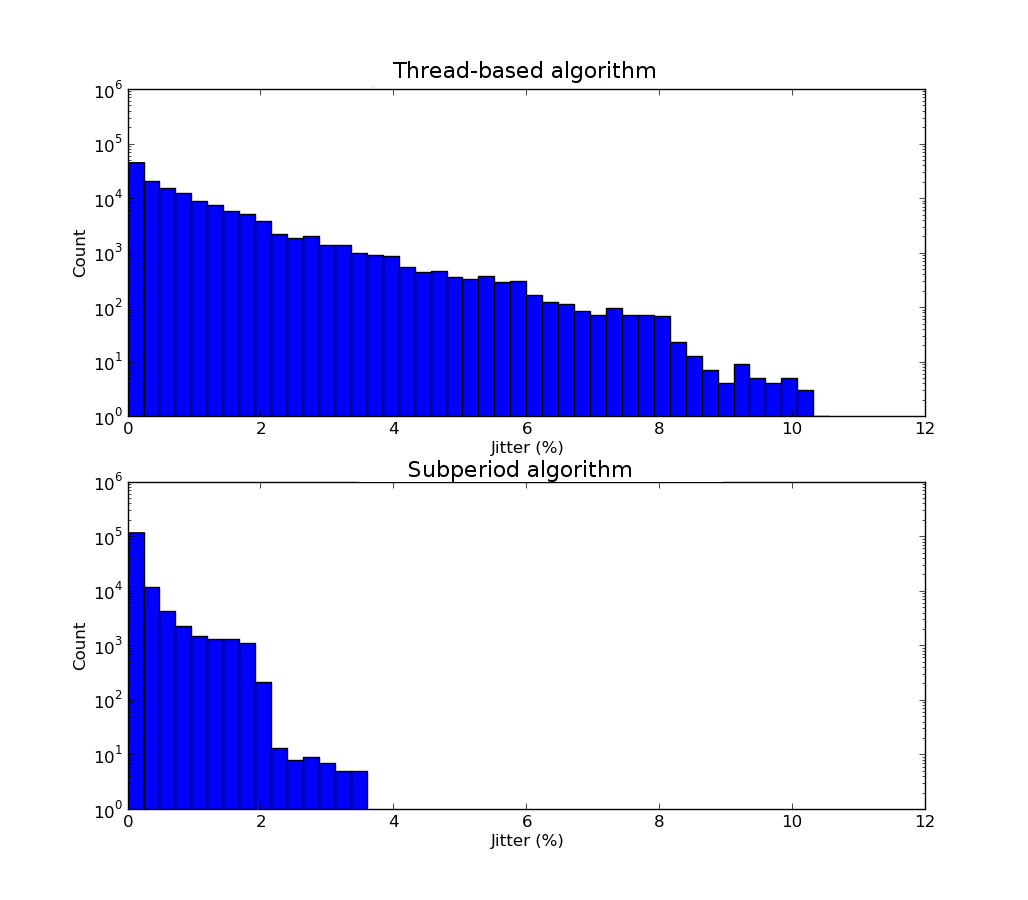
\includegraphics[scale=0.55]{Images/jitter_histo.png}
\caption[Jitter histograms.]{Jitter histograms for the thread-based algorithm (above) and subperiod algorithm (below).}
\label{fig:jitter_histo}
\end{figure}

It can be noticed that the jitter is considerably smaller with our algorithm and that the thread-based algorithm actually does not satisfy the requirement to have jitter less than 10 percent.

\subsubsection*{Traffic shaping}

As we mentioned, we are interested in making traffic less bursty as it produces memory allocation spikes which cause stop-the-world garbage collector to run in applications written in Java. 

We ran an experiment with the same setup as before, we registered one subscriber for the IS server and we compared the pattern of the updates received by that subscriber for both scheduling algorithms. In figures \ref{fig:burstiness} an \ref{fig:burstiness_hires} we present the number of updates in the time unit for a resolution of 20ms and 1ms respectively. 

\begin{figure}
\centering
\begin{subfigure}[ht]{0.45\textwidth}
\centering
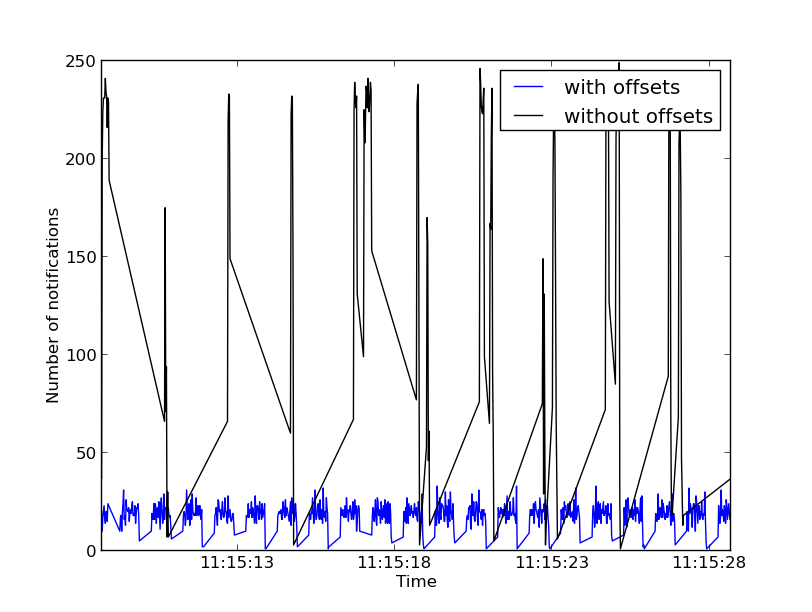
\includegraphics[width=\textwidth]{Images/burstiness.png}
\caption{Traffic burstiness comparison (low granularity).}
\label{fig:burstiness}
\end{subfigure}
~
\begin{subfigure}[ht]{0.45\textwidth}
\centering
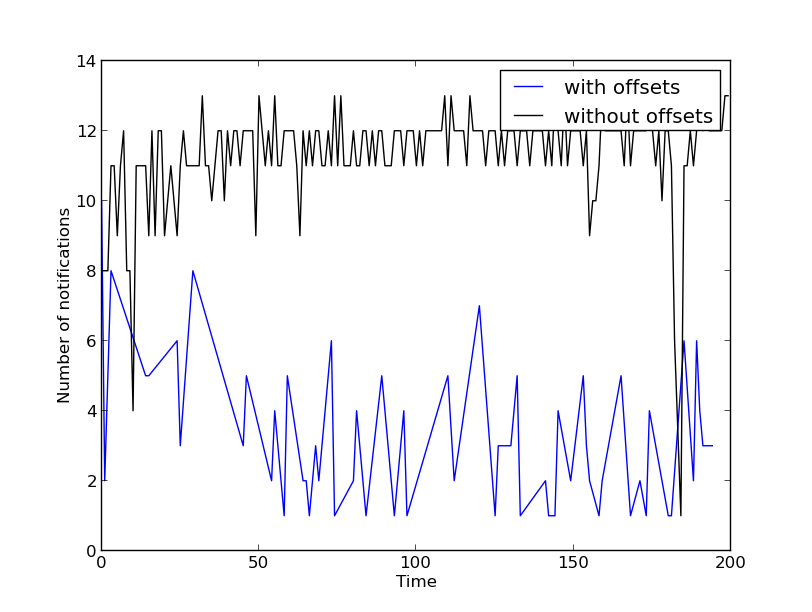
\includegraphics[width=\textwidth]{Images/burstiness_hires.png}
\caption{Traffic burstiness comparison during a high-load period.}
\label{fig:burstiness_hires}
\end{subfigure}
\label{fig:burstiness_both}
\caption{Traffic burstiness.}
\end{figure}

One can see that both the subperiod algorithm and randomization contribute to reduce the size of the traffic spikes. 

\subsubsection*{Global scheduling}

We repeated the simulation experiment for the global scheduling in the testbed. The setup was similar: 400 applications running on 40 nodes that publish one histogram in a time slot. The size of the histogram was chosen according to the three size classes identified in table \ref{tab:histosize}. 

We can see that the figure \ref{fig:one_slot_tbed} follows the same pattern as figures \ref{fig:one_slot_sim_latency} and \ref{fig:one_slot_sim_skew}. The only difference is the case of the large histogram when the IS server experiences bigger latencies under heavy load.

\begin{figure}[ht]
\centering
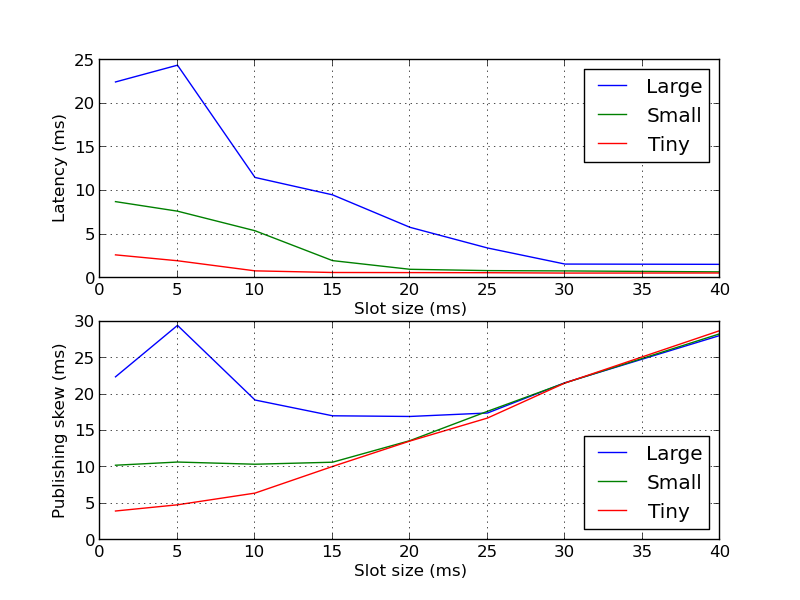
\includegraphics[scale=0.6]{Images/one_slot_tbed.png}
\caption{Latency and publishing skew vs. initial delay bound (testbed).}
\label{fig:one_slot_tbed}
\end{figure}

\subsubsection*{Throughput, latency and publishing skew}






